\documentclass{article}
\usepackage[utf8]{inputenc}

\title{PC Project Report}
\author{Liron Mizrahi}
\date{October 2016}

\usepackage{natbib}
\usepackage{graphicx}
\usepackage{algorithm2e}
\usepackage{subcaption}

\setlength{\parindent}{0em}
\setlength{\parskip}{1em}
\begin{document}

\maketitle

\section{Introduction}
K-means is  one of the simplest unsupervised learning algorithms to solve a clustering problem. Clustering is the process of partitioning a group of data points into a small number of clusters. In general, a cluster is defined as a set of similar objects. The similarity in a given set may vary according to data, therefore a clustering algorithm that finds an optimization in one set of data may not find an optimization in another set of data.

There are many variations of the k-means clustering algorithm, however we have looked at 2 of them, namely the normal k-means clustering and online k-means clustering.

\section{Terminology and definitions}
For this report we will define some terms and variables which will be used:
There is a dataset $S \in R^m$.\\
$\underline{x}$ is a data point in $S$.\\
$k$ is the number of clusters.\\
$\underline{\mu_j}$ is a cluster centre.\\
$d(\underline{x}, \underline{\mu_j})$ is the distance from $\underline{x}$ to $\underline{\mu_j}$.\\
$N_j$ is the number of points in cluster $j$.\\
The sum of squared error is given by:
    $$\sum_{j}\sum_{\underline{x}} || \underline{x} - \underline{\mu_j} ||^2 $$
where $||\cdot||$ is the Euclidean distance.\\
$\eta$ is the learning rate where $\eta \in \big[0, 1\big]$. The learning rate is used for the online k-means. It is used to increase or decrease the shift of the centres for each iteration.



\section{Background Theory}
As stated, k-means is a solution technique to solve a clustering problem. Clustering is the task of grouping a set of objects in such a way that objects in the same group have more similarities to each other than to those in other groups. Clustering is not just one specific algorithm, but it is a problem to be solved. The idea of a cluster cannot be precisely defined, as such different variations of the solution can be derived depending on the idea used of what constitutes a cluster and the method used to find them. This is one of the reasons why there are so many different clustering algorithms. Different cluster models are used by different people depending on their needs, and for each of these cluster models again different algorithms can be given. The cluster model used by k-means is called a centroid model, where each cluster is represented by a single mean vector.

\section{The Clustering Problem}
In centroid clustering, clusters are represented by a vector, which may not necessarily be a member of the dataset. When the number of clusters is fixed to $k$, k-means clustering becomes an optimization problem,i.e. find the $k$ cluster centers and assign the points to the nearest cluster center, such that the squared distances from the cluster are minimized, i.e. the sum squared error is minimized. This problem is known to be NP-Hard.


\newpage


\section{Algorithms}
Shown below is the pseudo-code for the k-means clustering algorithm and the Online k-means clustering algorithm:

\begin{algorithm}[H]
\SetAlgoLined
 Given dataset $S$ in $R^m$\;
 Choose $k$, which is number of clusters\;
 Choose the $k$ cluster centres(Randomly): $\underline{\mu_1}, \underline{\mu_2}, \dots, \underline{\mu_k}$\;
 \While{stopping condition does not hold}{
  \For{each $\underline{x} \in S$}{
    Find $min\big\{d(\underline{x}, \underline{\mu_1}), d(\underline{x}, \underline{\mu_2}), \dots, d(\underline{x}, \underline{\mu_k})\big\}$\;
    Say $d(\underline{x}, \underline{\mu_j})$ is the minimum\;
    Assign $\underline{x}$ to cluster $j$\;
  }
  
  \For{each cluster centre $\underline{\mu_j}$ }{
    move cluster centre to the mean of the points in its cluster\;
    $$\underline{\mu_j} \leftarrow \frac{1}{N_j} \sum_{\underline{x}}{\underline{x}} $$
    where $N_j$ is the number of points in cluster $j$.
  }
 }
 \caption{k-means clustering algorithm}
\end{algorithm}

\begin{algorithm}[H]
\SetAlgoLined
 Given dataset $S$ in $R^m$\;
 Choose $k$, which is number of clusters\;
 Choose the $k$ cluster centres(Randomly): $\underline{\mu_1}, \underline{\mu_2}, \dots, \underline{\mu_k}$\;
 \While{stopping condition does not hold}{
  \For{each $\underline{x} \in S$}{
    Find $min\big\{d(\underline{x}, \underline{\mu_1}), d(\underline{x}, \underline{\mu_2}), \dots, d(\underline{x}, \underline{\mu_k})\big\}$\;
    Say $d(\underline{x}, \underline{\mu_j})$ is the minimum\;
    Update $\underline{\mu_j}$\;
    $$\underline{\mu_j} \leftarrow \underline{\mu_j} + \eta(\underline{x} - \underline{\mu_j})$$
    where $\eta$ is the learning rate.
  }
  Decrease $\eta$ (This is an extra stopping condition).
  
 }
 \caption{Online k-means clustering algorithm}
\end{algorithm}

The stopping conditions may vary by time or by iterations. However, we have chosen the stopping condition to be bounded by the number of iterations.

\begin{figure}
    \begin{subfigure}{0.5\textwidth}
        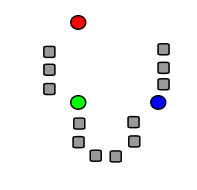
\includegraphics[width=0.9\linewidth, height=5cm]{Pictures/K_Means_Example_Step_1.png}
        \caption{ $k$ initial centres are randomly\\ generated (in this case k=3).}
    \end{subfigure}
    \begin{subfigure}{0.5\textwidth}
        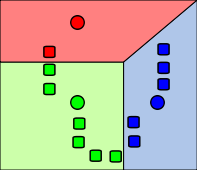
\includegraphics[width=0.9\linewidth, height=5cm]{Pictures/K_Means_Example_Step_2.png}
        \caption{ $k$ clusters are created by associating every data point with the nearest centre.}
    \end{subfigure}
    \begin{subfigure}{0.5\textwidth}
        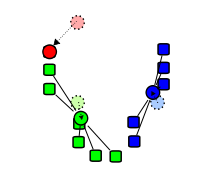
\includegraphics[width=0.9\linewidth, height=5cm]{Pictures/K_Means_Example_Step_3.png}
        \caption{The centre of each of the $k$ clusters\\ becomes the new mean of the points.}
    \end{subfigure}
    \begin{subfigure}{0.5\textwidth}
        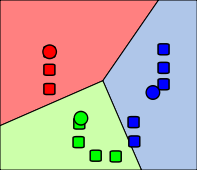
\includegraphics[width=0.9\linewidth, height=5cm]{Pictures/K_Means_Example_Step_4.png}
        \caption{Steps (b) and (c) are repeated until convergence has been reached.}
    \end{subfigure}
\caption{Example demonstrating how k-means works}

\end{figure}

\section{k-means vs Online k-means}





\end{document}
